\begin{enumerate}
\item If the probability of an event $E$ happening is $0.023$,then $P(\overline{E})=\underline{\hspace{2cm}}$.
\item Read the following passage and answer the questions given at the end:\newline\textbf{Diwali Fair}\newline A game in booth Diwali Fair involves using a spinner first.Then,if the spinner stops on an even member,the player is allowed to pick a marble from a bag.The spinner and the marbles in the bag are represented in \figref{fig:PROB.PNG}.\newline Prizes are given,when a block marble is picked.Shooter plays the game once.
\begin{figure}[H]
\centering
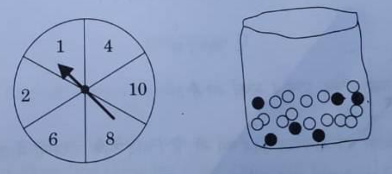
\includegraphics[width=\columnwidth]{figs/PROB.PNG}
\caption{A bag contains of marbles}
\label{fig:PROB.PNG}
\end{figure}

\item what is the probability that she will be allowed to pick a mobile from the bag$?$
\item suppose she is allowed to pick a marble from the bag,what if the probability of getting a prize,when it is given that the bag contains $20$ balls out of which $6$ came black$?$

\end{enumerate}
